\documentclass[a4paper]{article}

\usepackage[left=2cm, right=2cm, top=3cm, bottom=3cm]{geometry}
\usepackage[T1]{fontenc}
\usepackage{hyperref}
\usepackage{bookmark}
\usepackage{booktabs}
\usepackage{float}
\usepackage[linesnumbered,ruled,vlined]{algorithm2e}
\hypersetup{
    linktoc=all,
    linkcolor=blue,
    colorlinks=true
}
\usepackage{amsmath}
\usepackage{float}
\usepackage{graphicx}
\usepackage{subcaption}
\restylefloat{figure}

\usepackage[english]{babel}
\usepackage{tocloft}

\usepackage{fancyhdr}
\pagestyle{fancy}
\fancyhf{}
\fancyhead[L]{Algorytmy ewolucyjne}
\fancyhead[R]{Paweł Pozorski}
\fancyfoot[C]{\thepage}

\renewcommand{\normalsize}{\fontsize{9}{11}\selectfont}
\normalsize

\title{
    \textbf{I}ndoor \textbf{O}utdoor \textbf{Net} \\
    \textit{Creation report and performance analysis} \\}
\author{Paweł Pozorski \\ Warsaw University of Technology}
\date{June 5, 2025}

\begin{document}

\maketitle
\begin{abstract}
    Following report contains description of the process of creating IO Net, a neural network architecture designed for indoor and outdoor image classification. The report includes details on the dataset used - from retrieval and choice of publicly available datasets up to description on creation of artificial dataset based on WikiMedia Image Dataset (WIT). The architecture of the network, training process, and performance analysis are also discussed. The report concludes with a summary of the results and potential future work.
\end{abstract}

\newpage
\tableofcontents
\newpage

\section{Introduction}

The goal of this project was to create a neural network architecture capable of classifying images into two categories: indoor and outdoor. The motivation behind this task is to develop a model that can effectively distinguish between these two environments, which has applications in various fields such as robotics, autonomous vehicles, and augmented reality. Such a model can be used in various low-resources environments, from  artificial driven drones and cars, up to mobile devices, where the ability to quickly and accurately classify images is crucial.

Therefore much effort has been put into creating a model that is not only accurate but also efficient in terms of computational resources. The architecture of the network has been designed to balance complexity and performance, ensuring that it can be deployed in real-world applications without requiring excessive computational power.

Entire work is limited to publicly available datasets and models architectures. Limited training resources has forced this work to be developed under online learning ideology, with $2$ industry leading architectures fine tuned for our cause (refer to section \ref{sec:models}). The datasets has been chosen based on prior research on similar tasks, however limitation of their size and quality has been taken into account leading to creation of an artificial dataset based on WikiMedia Image Dataset (WIT). The dataset is described in detail in section \ref{sec:datasets}.

\section{Datasets}
\label{sec:datasets}

\subsection{Online datasets}

For initial fine tuning of the model online datasets have been used, as they carry little to none risk of mislabeling and are well documented. The datasets used in this project shown in table \ref{tab:datasets}. Some of them have been used in similar tasks (refer to \href{https://huggingface.co/prithivMLmods/IndoorOutdoorNet}{Indoor Outdoor Net on Huggging Face}), while others have been chosen based on their size and quality. The datasets are publicly available and can be accessed through the provided links. All images have been reshaped to $224 \times 224$ pixels and converted to RGB format. The datasets have been split into training, validation, and test sets, with the training set containing the majority of the images. They all have been saved together to form final dataset referred as \textit{other datasets} in the rest of projects notebooks.

\begin{table}[H]
    \centering
    \caption{Datasets Information}
    \label{tab:datasets}
    \begin{tabular}{@{}lllll@{}}
        \toprule
        \textbf{Field}  & \href{https://huggingface.co/datasets/prithivMLmods/IndoorOutdoorNet-20K}{\textbf{Indoor Outdoor Net Dataset}} & \href{https://www.kaggle.com/datasets/itsahmad/indoor-scenes-cvpr-2019}{\textbf{MIT Indoor Scenes}} & \href{https://www.kaggle.com/datasets/arnaud58/landscape-pictures}{\textbf{Landsaping Pictures}} & \href{https://paperswithcode.com/dataset/ost300}{\textbf{OST 300}} \\ \midrule
        Total Images    & 19,998                                                                                                         & 15,619                                                                                              & 4,319                                                                                            & 10,324                                                             \\
        Size            & $\sim$451 MB                                                                                                   & 2.34 GB                                                                                             & 620 MB                                                                                           & $\sim$3.5 GB                                                       \\
        Train size      & 15,998                                                                                                         & 12,495                                                                                              & 3,455                                                                                            & 8,259                                                              \\
        Validation size & 2,000                                                                                                          & 1,562                                                                                               & 432                                                                                              & 1,032                                                              \\
        Test size       & 2,000                                                                                                          & 1,562                                                                                               & 432                                                                                              & 1,033                                                              \\
        Classes         & Indoor, Outdoor                                                                                                & Indoor                                                                                              & Outdoor                                                                                          & Outdoor                                                            \\
        \bottomrule
    \end{tabular}
\end{table}

\begin{figure}[H]
    \centering
    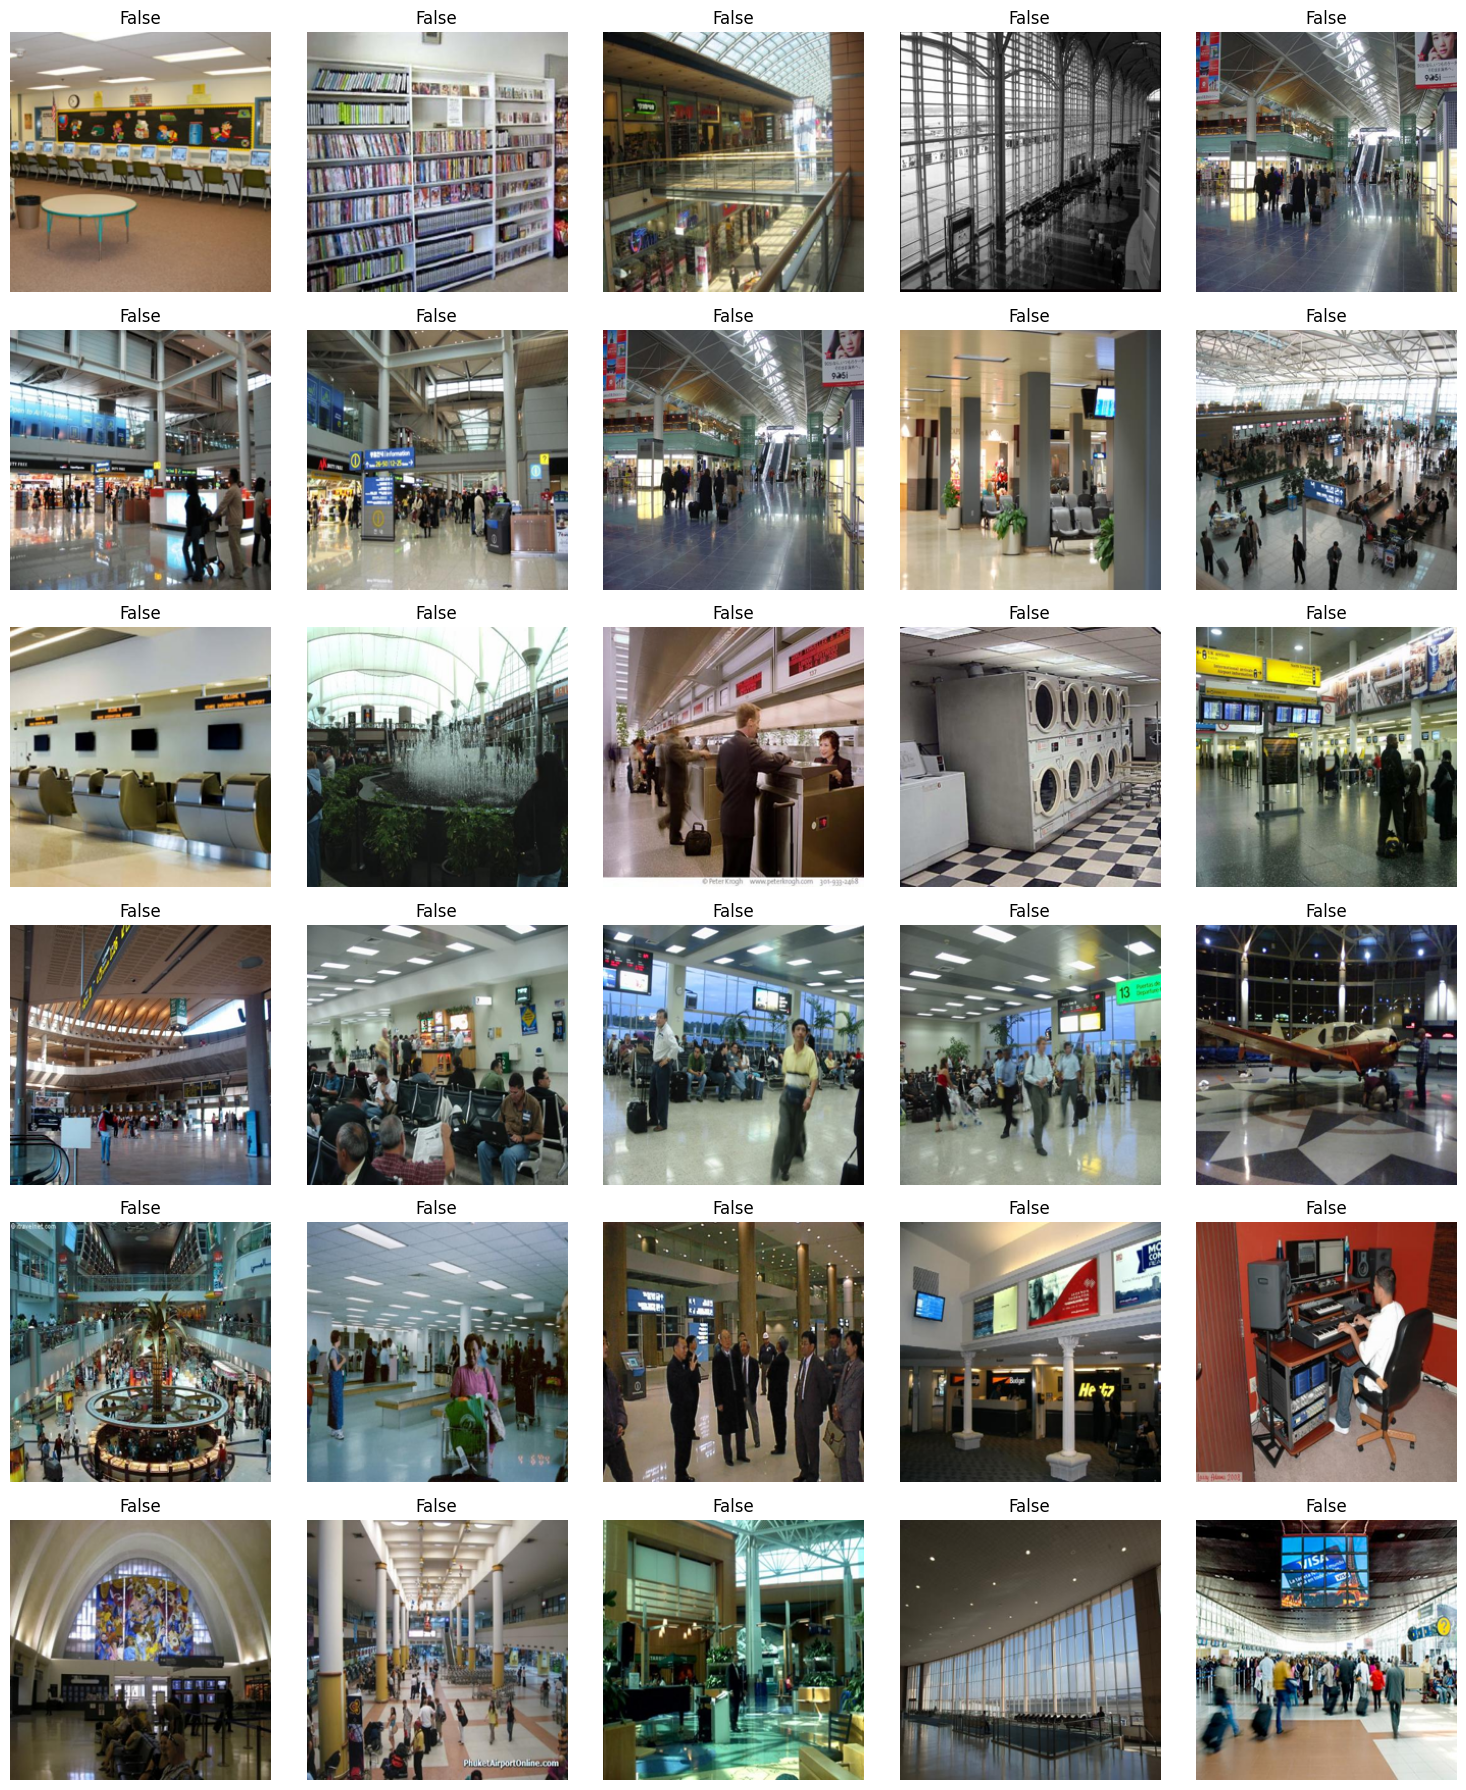
\includegraphics[width=0.4\textwidth]{images/indoor-outdoor-20k.png}
    \caption{Example images from \href{https://huggingface.co/datasets/prithivMLmods/IndoorOutdoorNet-20K}{\textbf{Indoor Outdoor Net Dataset}} alongside their labels.}
\end{figure}

\begin{figure}[H]
    \centering
    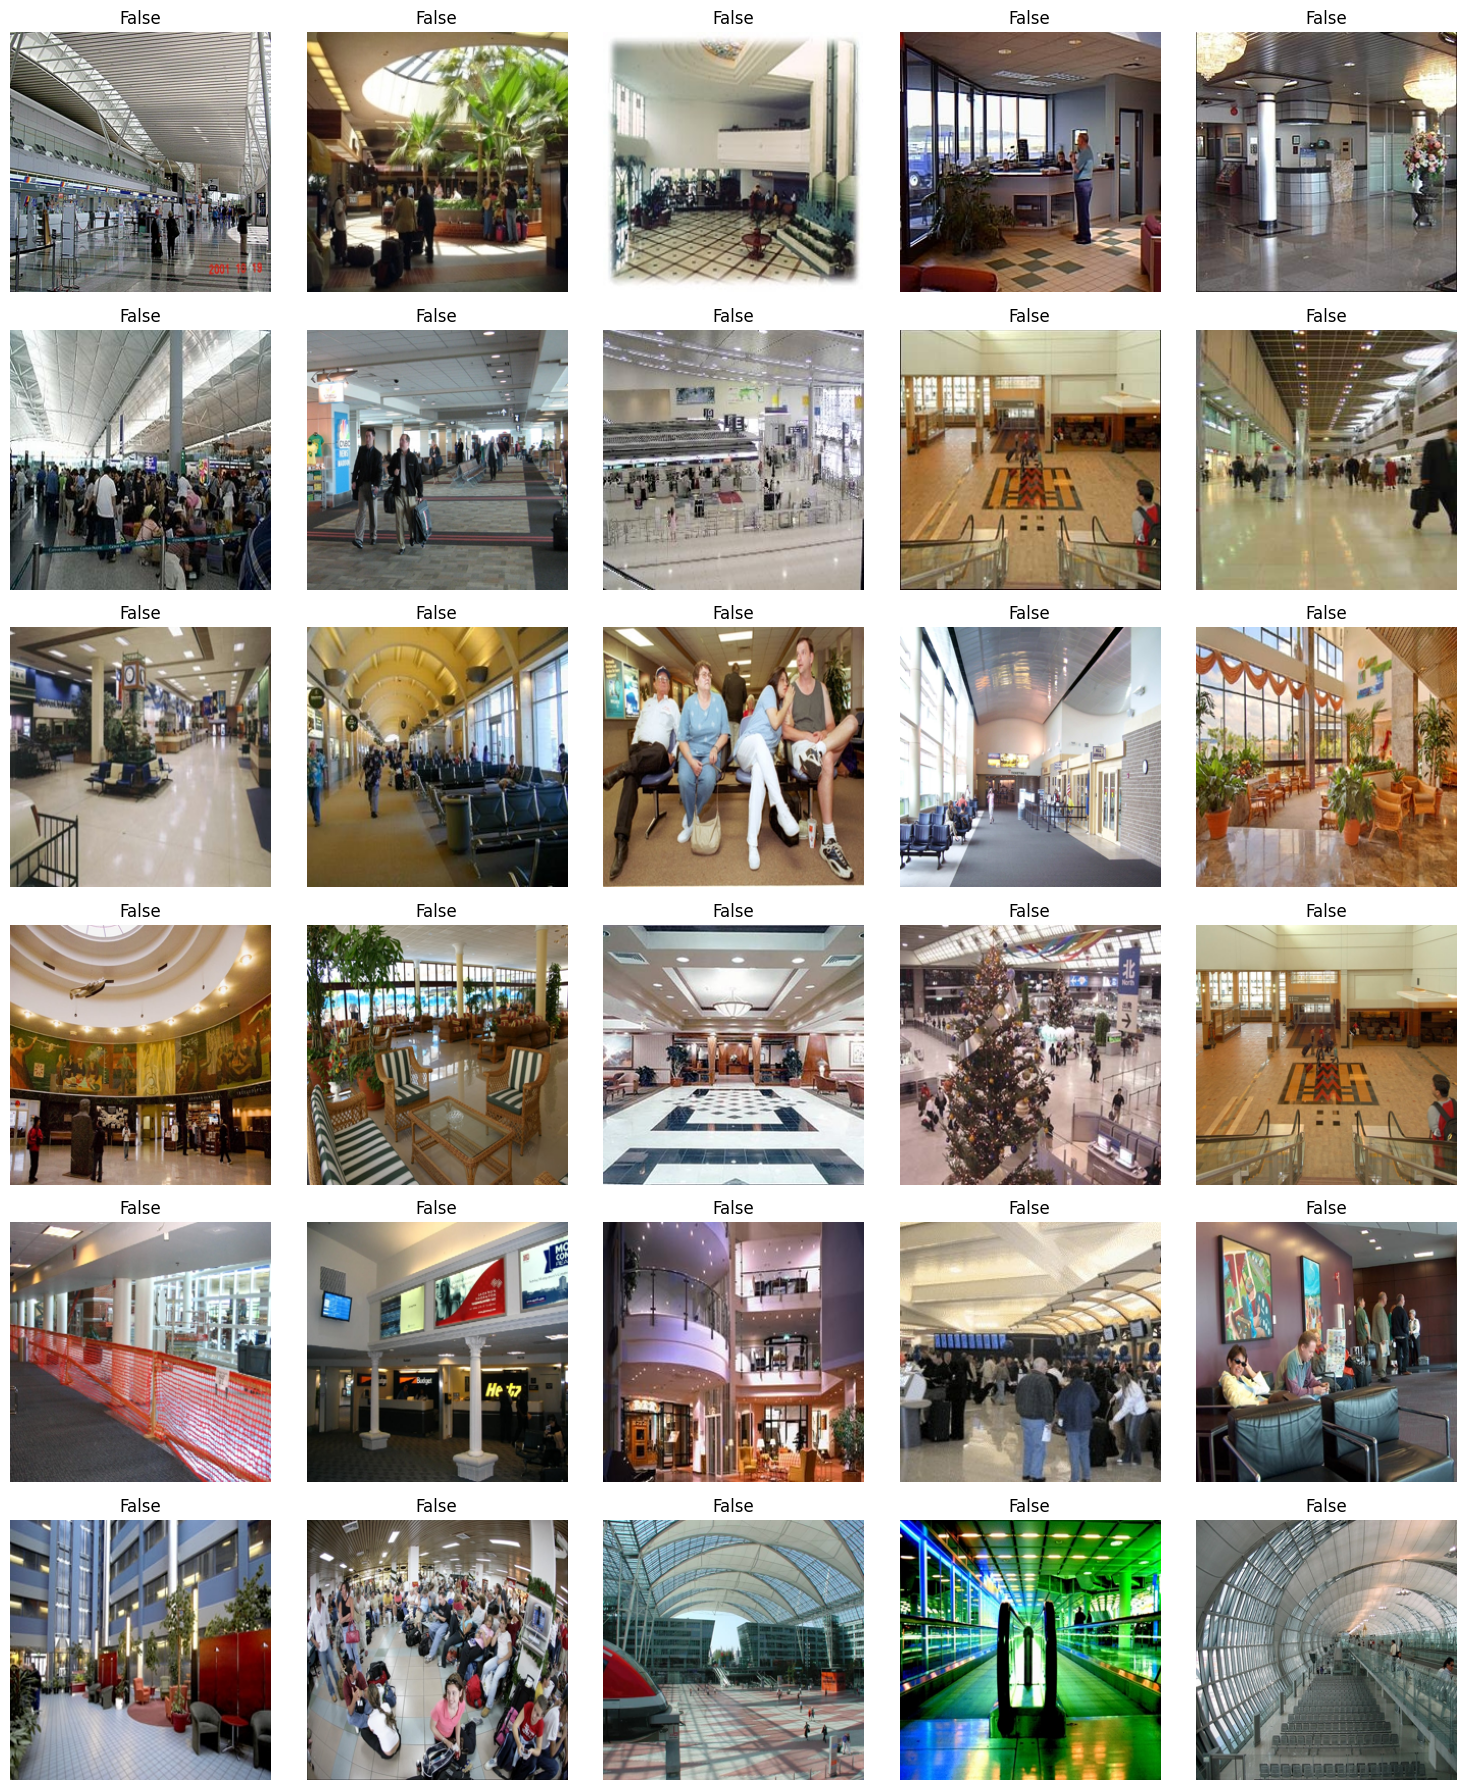
\includegraphics[width=0.4\textwidth]{images/mit-indoor-scenes.png}
    \caption{Example images from \href{https://www.kaggle.com/datasets/itsahmad/indoor-scenes-cvpr-2019}{\textbf{MIT Indoor Scenes}} alongside their labels. They look very similar to \textit{Indoor Outdoor Net Dataset}, however they contain only indoor images. There are some not obvious images containing trees or large staircases.}
\end{figure}

\begin{figure}[H]
    \centering
    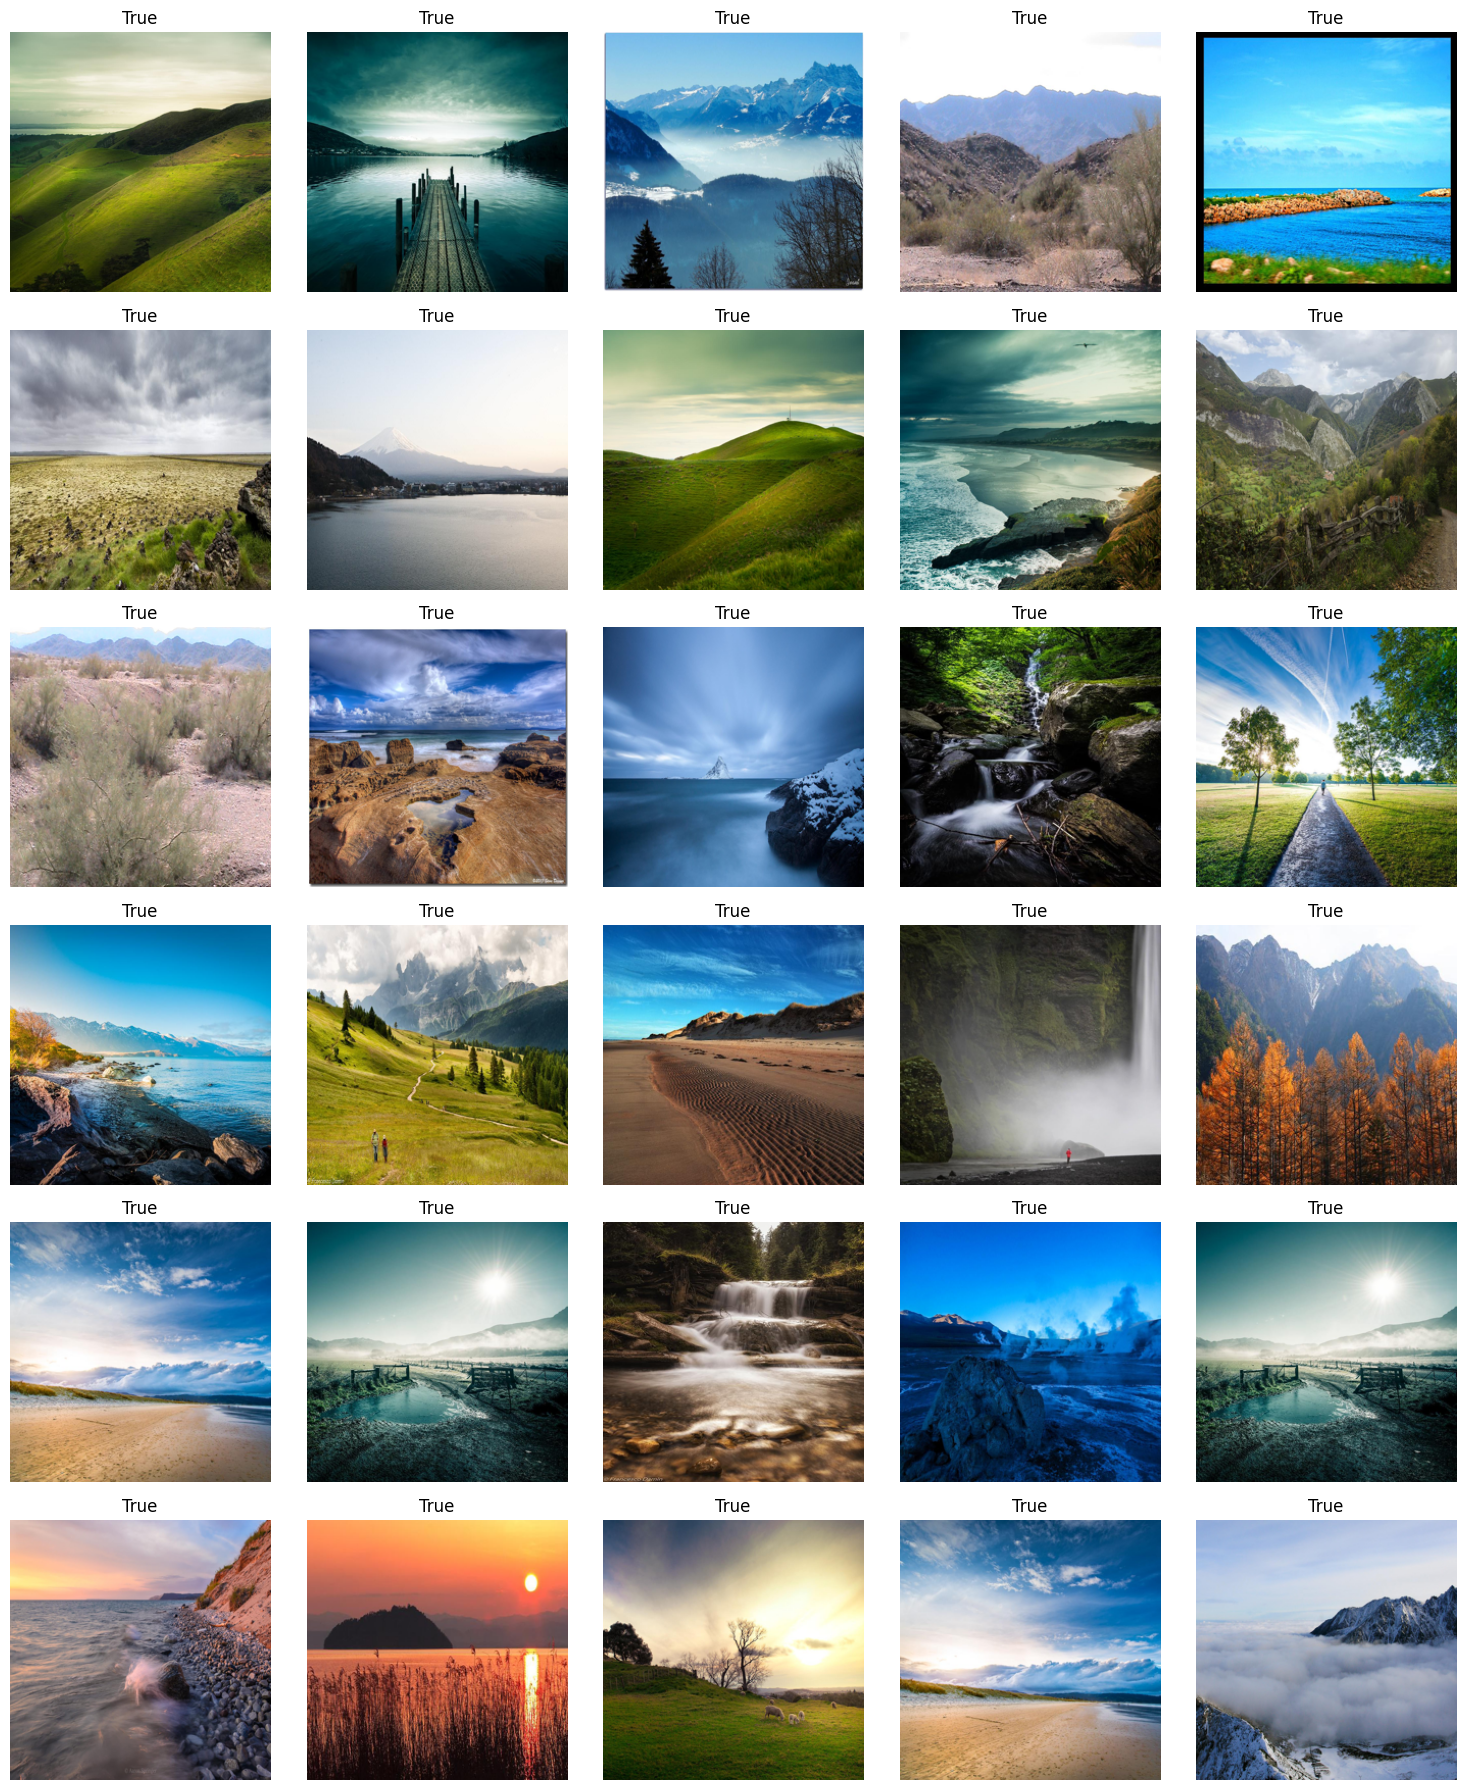
\includegraphics[width=0.4\textwidth]{images/landscaping-pictures.png}
    \caption{Example images from \href{https://www.kaggle.com/datasets/arnaud58/landscape-pictures}{\textbf{Landsaping Pictures}}alongside their labels. Most of they are expected to be very easy for the model to classify as outdoor. This dataset was brought to the project to increase the number of outdoor images and to allow model to learn correlation between outdoor images and nature.}
\end{figure}

\begin{figure}[H]
    \centering
    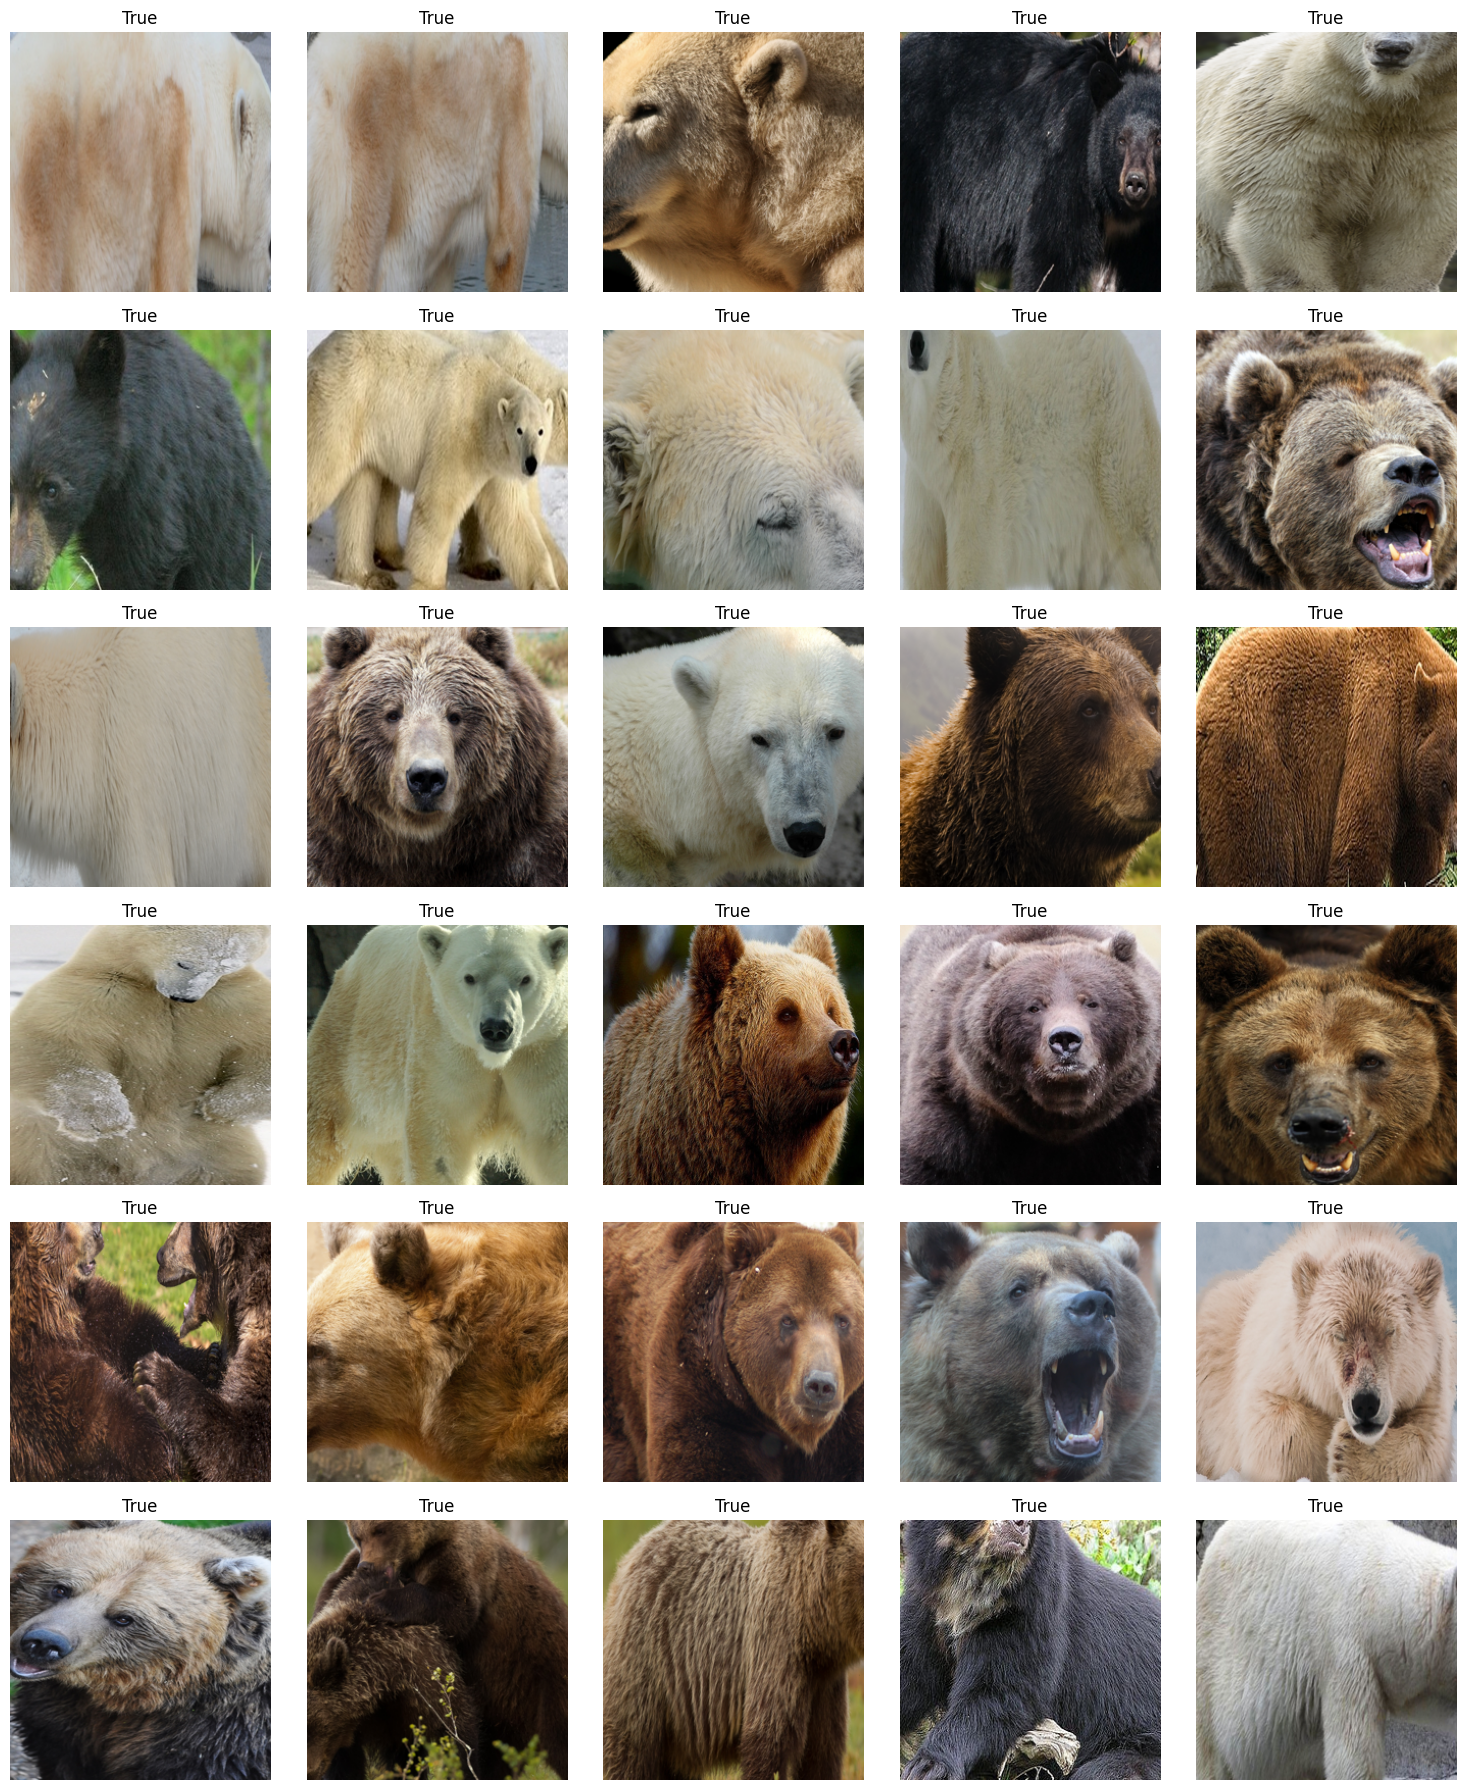
\includegraphics[width=0.4\textwidth]{images/ost-300.png}
    \caption{Example images from \href{https://paperswithcode.com/dataset/ost300}{\textbf{OST 300}} alongside their labels. This dataset contains images of 7 classes - \textit{animal, building, grass, mountain, plant, sky and water}. As shown on the picture, images within one class are not that diverse. To increase training speed they should be deduplicated, however it was not done in this project.}
\end{figure}

\subsection{WIT Images Dataset}

The WikiMedia Image Dataset (WIT) is a large-scale dataset containing images and their associated metadata from Wikimedia Commons. It is designed to provide a diverse set of images for various computer vision tasks, including image classification, object detection, and segmentation. The dataset contains millions of images, covering a wide range of categories and topics, however google publised their cleaned and limited version on \href{https://huggingface.co/datasets/google/wit}{Hugging Face}, with $11.5$ million of unique images, alongside with their metadata containing information about the image, such as its title, description, and categories in various languages, as well as the image embedding.

The main challenge in using WIT for this project was the lack of specific indoor and outdoor categories. The dataset contains a wide range of images, but it does not explicitly categorize them as indoor or outdoor. To address this issue, a detailed research was conducted to identify best performing algorithm for automatic classification of images into indoor and outdoor categories with smallest possible error rate.

\subsubsection{Automatic classification of images into indoor and outdoor categories using MLLMs}

MLLMs (Multimodal Large Language Models) have shown promising results in various computer vision tasks, including image classification. In this project, MLLMs were used to automatically classify images from the WIT dataset into indoor and outdoor categories. Due to limited resources and enormous size of the dataset, only small models were used (refer to table \ref{tab:mlm_models}). All models were provided with fixed following prompt:

\begin{quote}
You are a helpful assistant. You will be given an image and its description.
Your task is to return one digit indicating if image shows outdoor or indoor scene.

For outdoor scene return 1, for indoor scene return 0. If image depicts neither, return N.

For example, if the image shows a person in a park, return 1.
If an image shows a person in a room, return 0.
If the image is not clear, return N. If image is a photo of an map, return N.
Try your best not to return N.

Think twice before answering, I really need this for my research. I believe in you.
Remember to respond with a single digit, without any additional text or explanation.
\end{quote}

In order to make results reproducible, all calls were made with temperature set to $0.0$ and top-p set to $0.95$, with random seed set to $42$. Response tokens were limited to $1$ and answer was treated as valid only if it was either $0$, $1$ or $N$. They were all asked to label first $1000$ images from WIT dataset. Their responses were collected and analyzed. The results of the classification are shown in table \ref{tab:mlm_results}. Individual image label was considered correct if all models returned the same label. Only $295$ out of $1000$ images fulfilled that condition, with majority of them considered to be outdoor. With that poor performance another model was tested (\textit{internvl3-8b-instruct}, Parameters: 8B, Year: 2023, Country: USA, Architecture: Multimodal Vision-Language Instruct Transformer). It returned $0$ for $63$ images, $1$ for $77$ images and $N$ for $860$ images. With significantly higher computation cost and no obvious improvement in results, it was decided not to use MLLMs for this task.

\begin{table}[H]
    \centering
    \caption{Information on Selected MLLM Models}
    \label{tab:mlm_models}
    \begin{tabular}{@{}lcccc@{}}
        \toprule
        \textbf{Model} & \textbf{Parameters} & \textbf{Year} & \textbf{Country} & \textbf{Architecture} \\ \midrule
        Qwen2.5-VL-3B-Instruct    & 3B   & 2023 & China  & Vision-Language Instruct Transformer \\
        google\_gemma-3-4b-it     & 4B   & 2022 & USA    & Transformer with Multimodal Adaptation \\
        internvl3-2b-instruct     & 2B   & 2023 & USA    & Multimodal Vision-Language Transformer \\ \bottomrule
    \end{tabular}
\end{table}

\begin{table}[H]
    \centering
    \caption{MLLM Classification Results}
    \label{tab:mlm_results}
    \begin{tabular}{@{}lccc@{}}
        \toprule
        Result  & Gemma & Qwen & Internvl3 \\ \midrule
        False   & 387   & 428  & 265 \\
        True    & 208   & 63   & 339 \\
        None    & 405   & 509  & 396 \\ \bottomrule
    \end{tabular}
\end{table}

\begin{figure}[H]
    \centering
    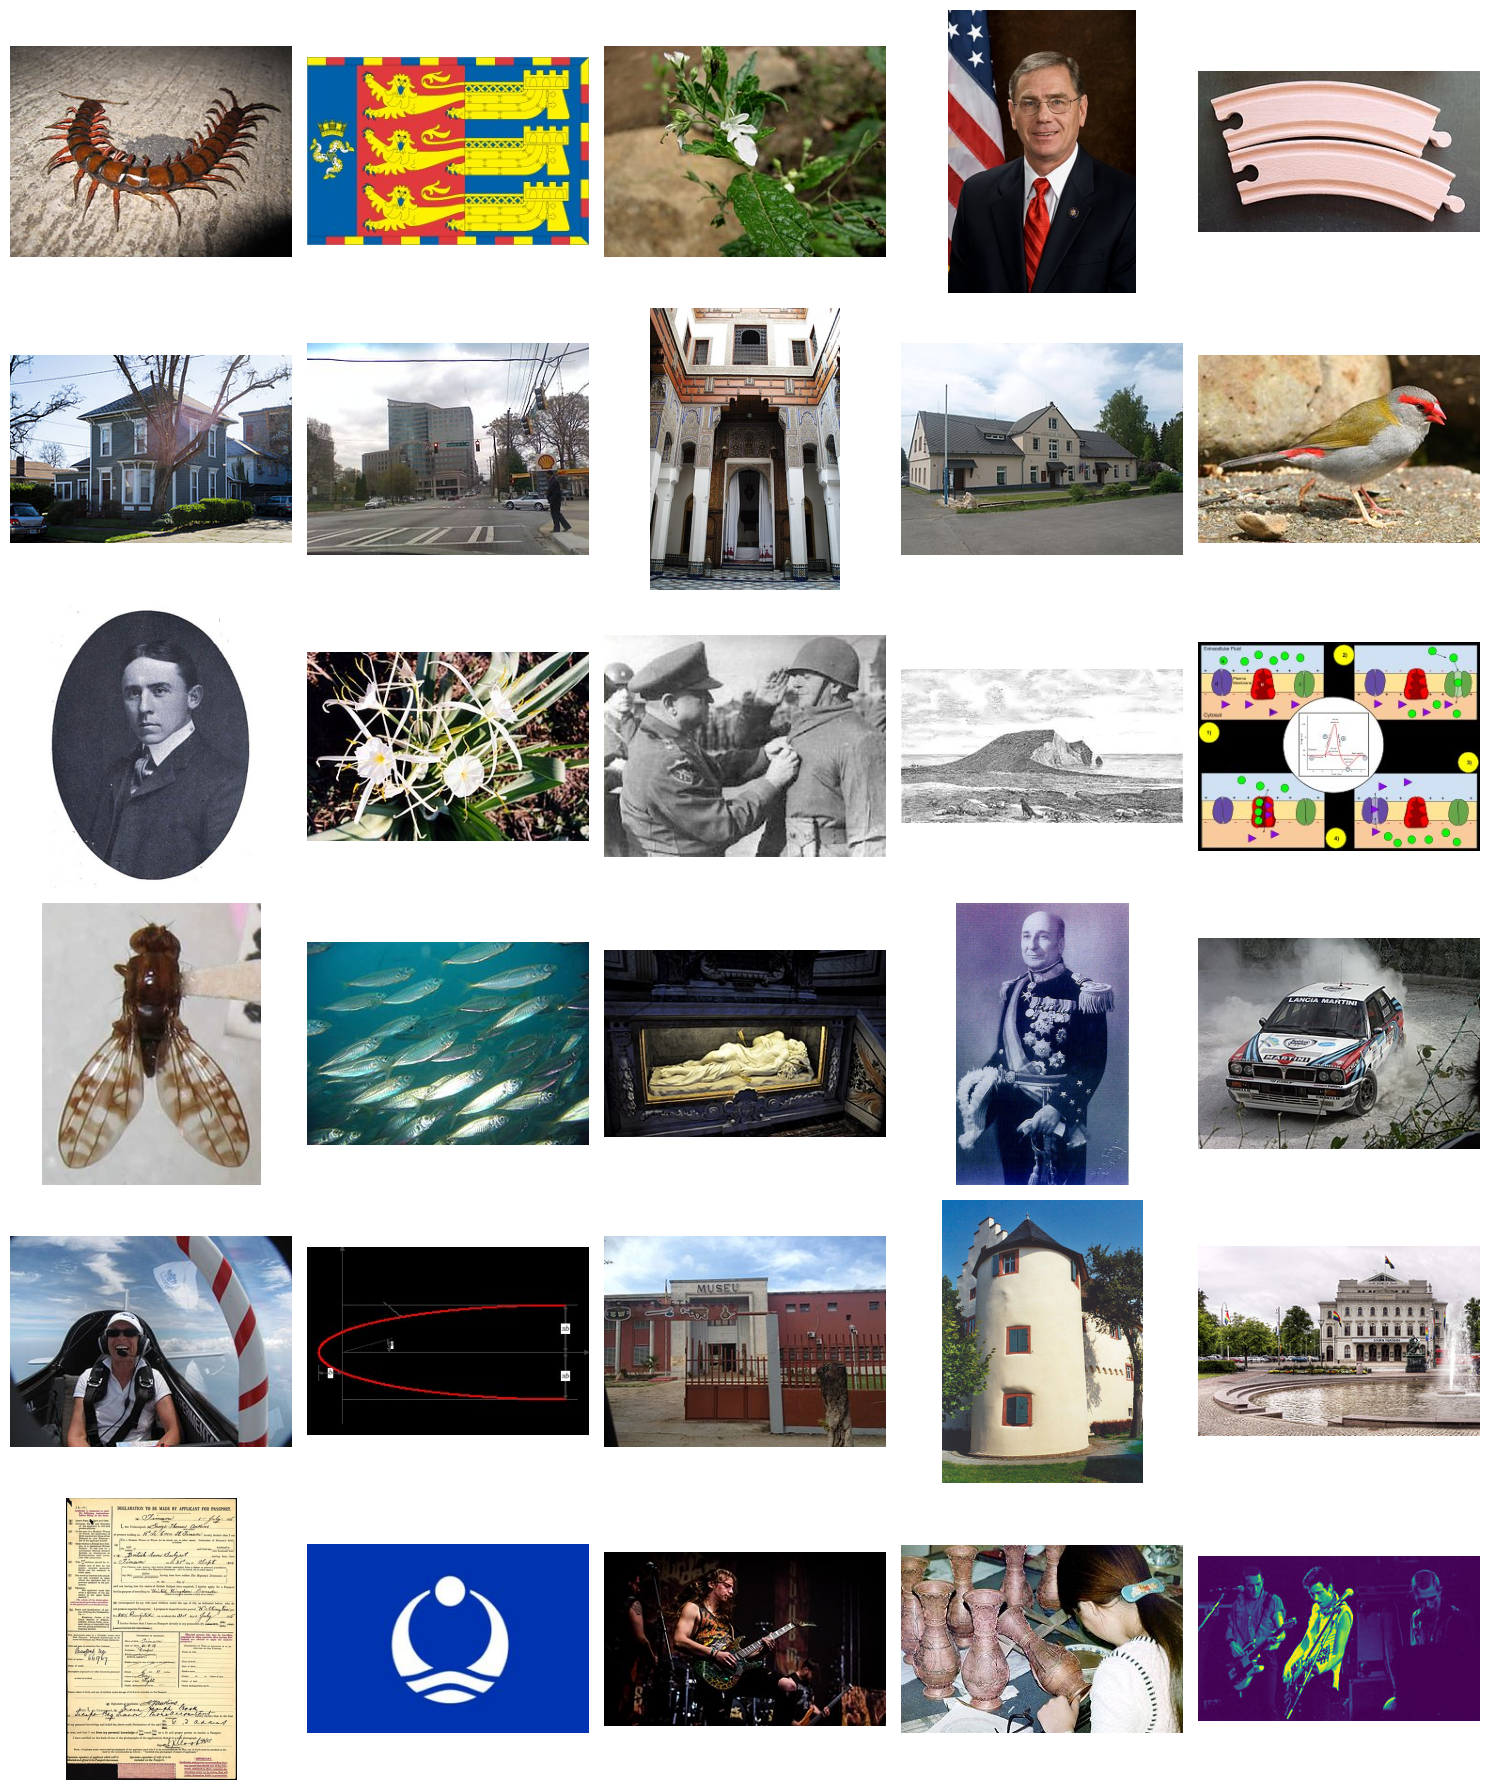
\includegraphics[width=0.4\textwidth]{images/invalid.png}
    \caption{Images that were considered invalid by MLLMs. There are in fact many noisy images present, but some of them depicts clearly outdoor scenes as buildings (or indoor as concerts). This proofs high FRR of MLLMs in this task.}
\end{figure}

\begin{figure}[H]
    \centering
    \begin{subfigure}[b]{\textwidth}
        \centering
        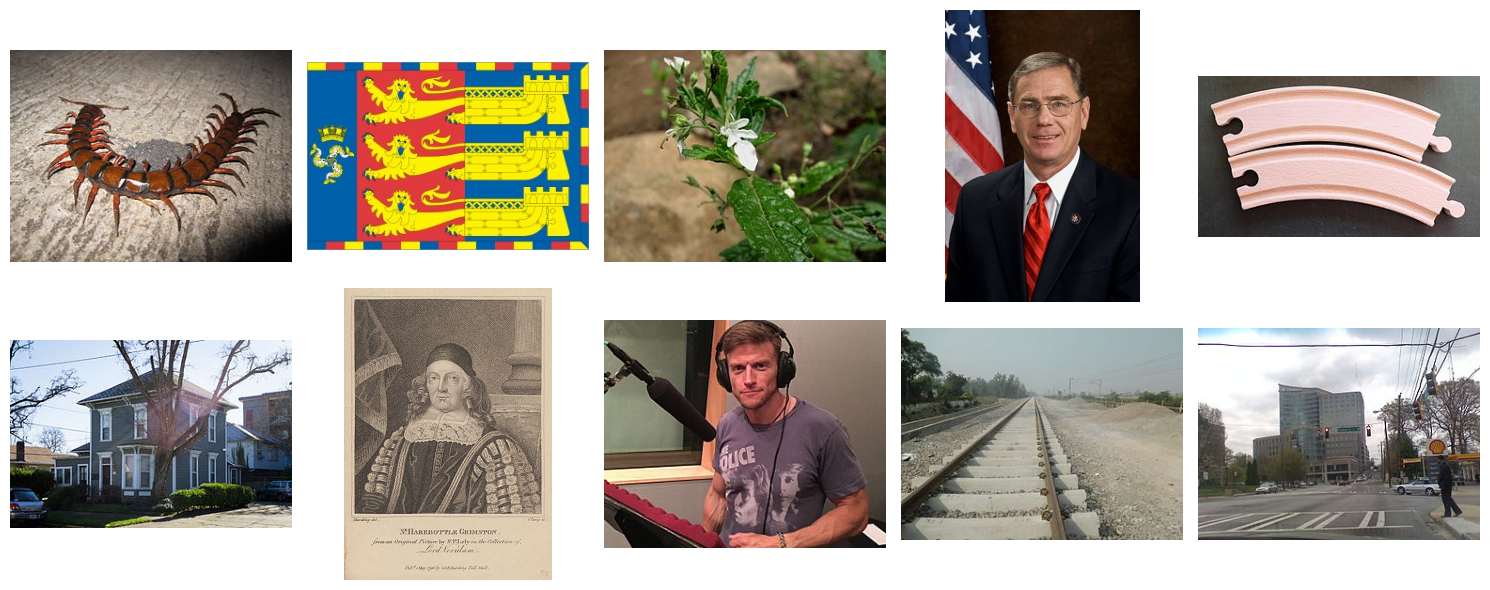
\includegraphics[width=0.7\textwidth]{images/mllm-indoor.png}
    \end{subfigure}

    \vspace{0.5cm}

    \begin{subfigure}[b]{\textwidth}
        \centering
        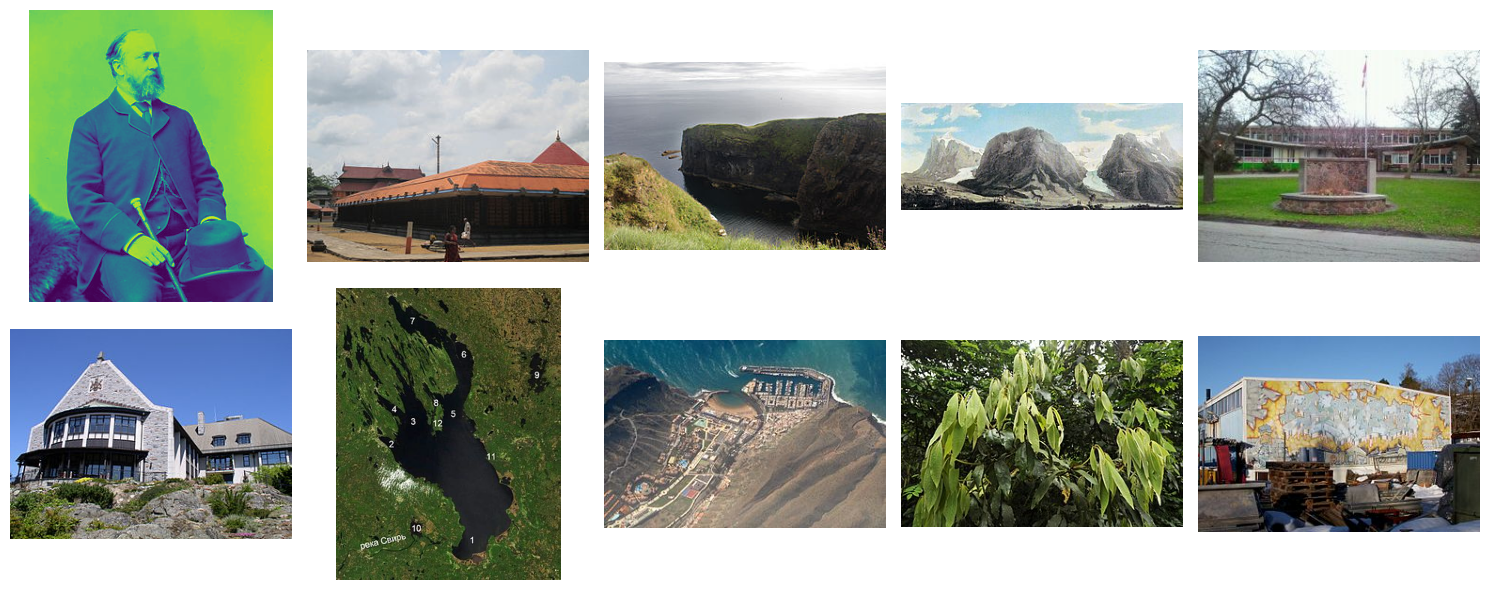
\includegraphics[width=0.7\textwidth]{images/mllm-outdoor.png}
    \end{subfigure}
    \caption{Comparison of MLLMs classification for indoor and outdoor scenes. Many outdoor scenes are misclassified as indoor, while indoor scenes are mostly classified correctly. This shows that MLLMs are not suitable for this task, however they can be used to filter out images that are not clearly indoor or outdoor.}
\end{figure}

\subsubsection{Automatic classification of images into indoor and outdoor categories using another architecture fine-tuned for this task}

Next approach was to use \textbf{Indoor Outdoor Net} architecture, which is a fine-tuned version of \textit{google/siglip2-base-patch16-224} for indoor and outdoor image classification. This model was trained on earlier mentioned dataset of $20,000$ images. In order to allow our final model to achieve performance superior to its direct predecessor, it was decided to use only images it classified with certainity of $0.9$ or higher. This way, the model was able to filter out images that were not clearly indoor or outdoor (irrelevant for our task) as well as to avoid images that could have been misclassified.

\begin{figure}[H]
    \centering
    \begin{subfigure}[b]{\textwidth}
        \centering
        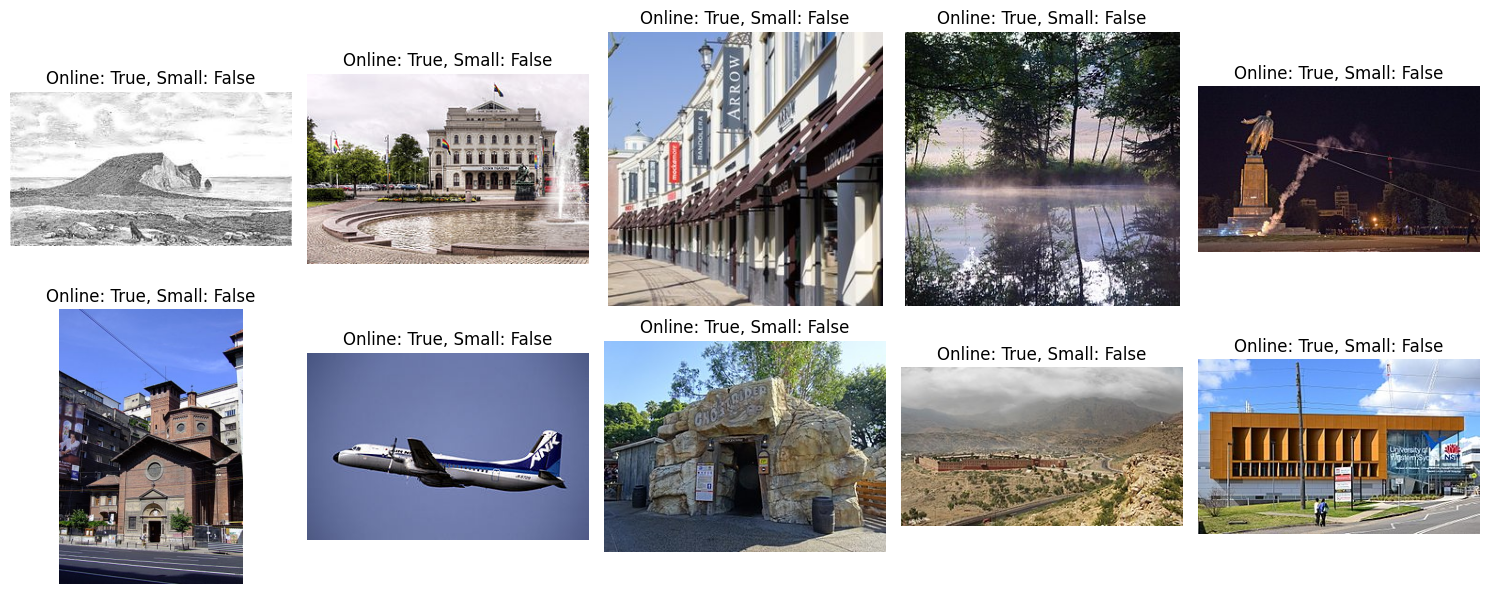
\includegraphics[width=0.7\textwidth]{images/small-online.png}
    \end{subfigure}

    \vspace{0.5cm}

    \begin{subfigure}[b]{\textwidth}
        \centering
        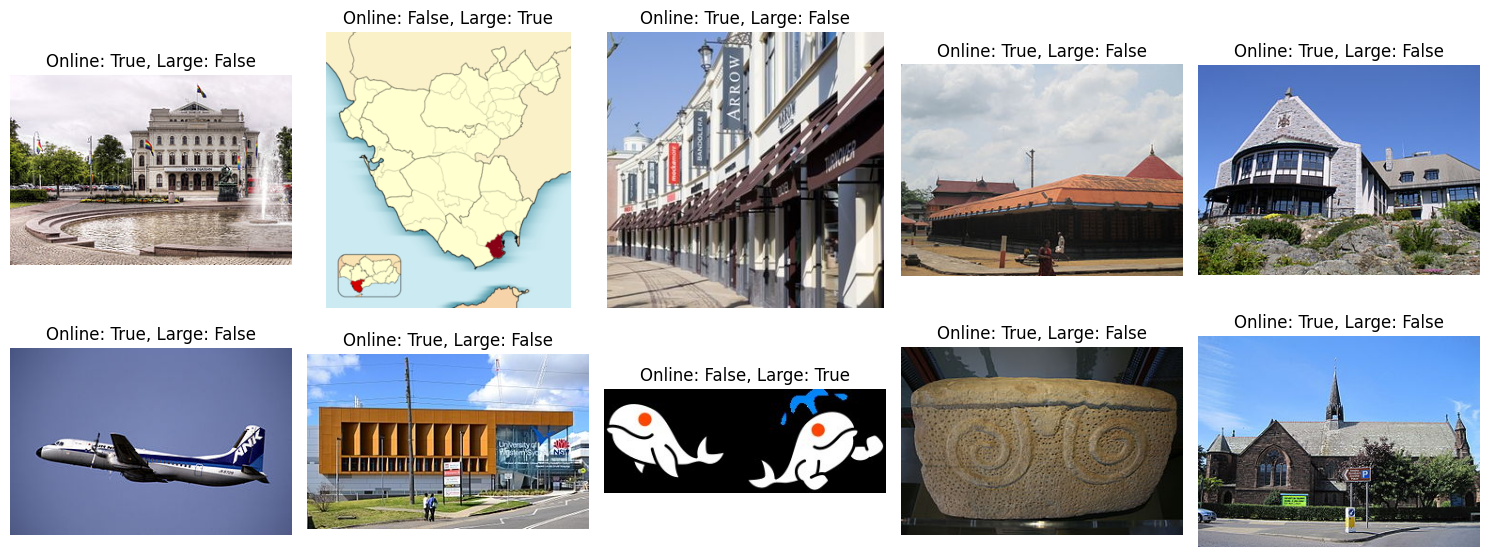
\includegraphics[width=0.7\textwidth]{images/large-online.png}
    \end{subfigure}
    \caption{Differences in label prediction of our ensemble of $3$ small MLLMs and Indoor Outdoor Net (above) and of \textit{internvl3-8b-instruct} and Indoor Outdoor net (below). Indoor Outdoor net label is called \textbf{Online}. Online net is always closer to correct answer, however another problem arises - there are many FARs as pictures of maps or animated images.}
\end{figure}

\begin{figure}[H]
    \centering
    \begin{subfigure}[b]{\textwidth}
        \centering
        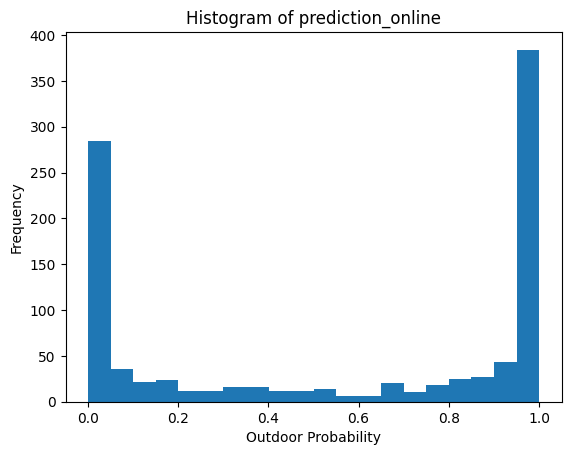
\includegraphics[width=0.3\textwidth]{images/histogram.png}
    \end{subfigure}

    \vspace{0.5cm}

    \begin{subfigure}[b]{\textwidth}
        \centering
        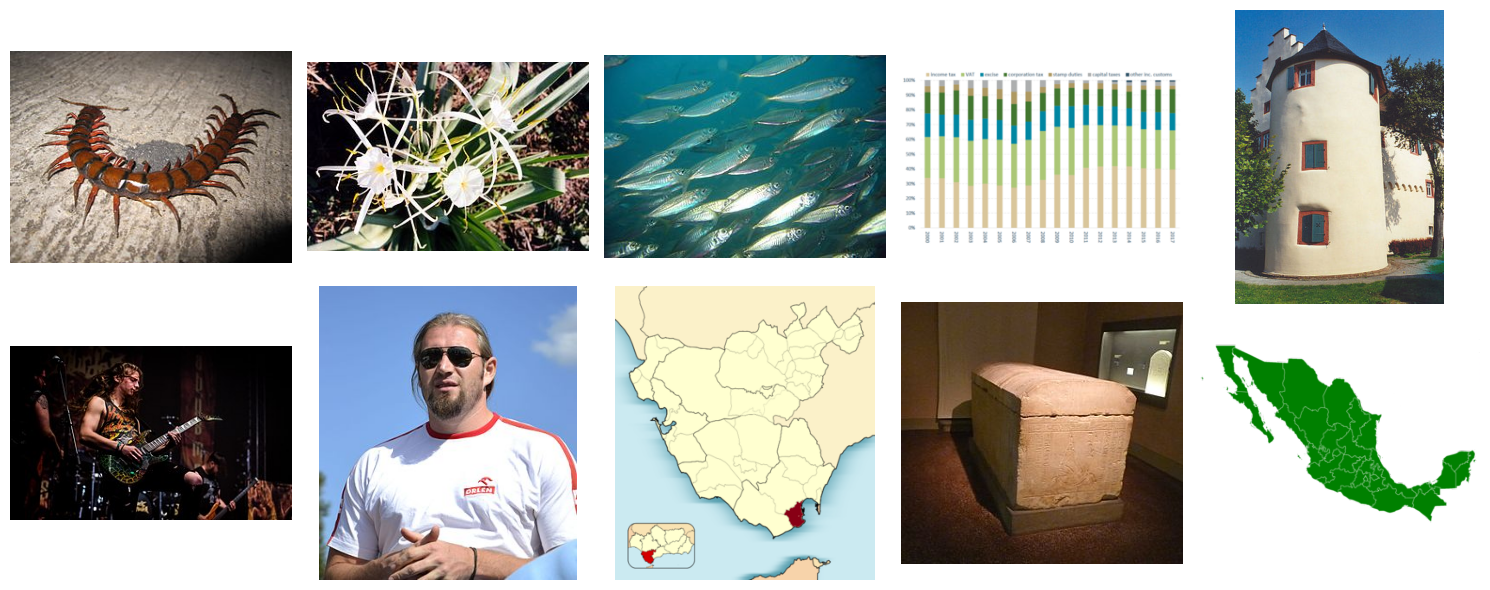
\includegraphics[width=0.6\textwidth]{images/deleted.png}
    \end{subfigure}
    \caption{Histogram of certainty of online model predictions. Cutof at $0.1$ will not delete that many images. Below are examples of such deleted images.}
    \label{fig:mllms_results}
\end{figure}

\subsubsection{Further processing}

Next step was to remove duplicated images based on their embeddings. For our exploratory set of $1000$ images, cosine similarity score was calculated between each pair of images and images with score above $0.9$ were considered duplicates. That lead to deletion of $4$ images. Moreover, broken images were detected and removed (ie. those with small number of unique pixels, or with no pixels at all). This lead to deletion of $3$ images.

Final preprocessing step was to remove images that are still not relevant for our task. That was compleated using \textit{openai/clip-vit-large-patch14} zero-shot classifier. It was used to classify images into $2$ classes: \textit{animated chart or infographic} and \textit{real photograph}. All images with first class label certaininty above $0.95$ were deleted. This lead to deletion of $ 78$ images out of first $300$ images accepted to that point, but globally this percentage proved to be way lower.

Finally the pipeline was crafted. It was labeling images in batches of $64$ (first reshape to $224\times224$ RGB), removing images with less than $10$ unique pixels. All images were gruopped  into super-batches of size same as files available on the source, and deduplication with threshold of $0.9$ was performed on each super-batch. Then noise removal was performed using zero-shot classifier, which removed images with labels \textit{animated chart or infographic} with certainity above $0.95$. $14$ files was processed in total, giving around $22.5$ gb of raw data in \textit{.npz} format ($169442$ individual images). Then global deduplication took place, removing $146$ images. At that point dataset contained $169296$ images, $55893$ of which were labeled as indoor and $113259$ as outdoor. To tackle this imbalance, \textbf{ENN} algorithm was used on first $951$ components of the embeddings ($90\%$ variance explained). This removed around $21\%$ of the images, leaving us with $133611$ images of classes indoor ($55893$) and outdoor ($77718$).

\begin{figure}[H]
    \centering
    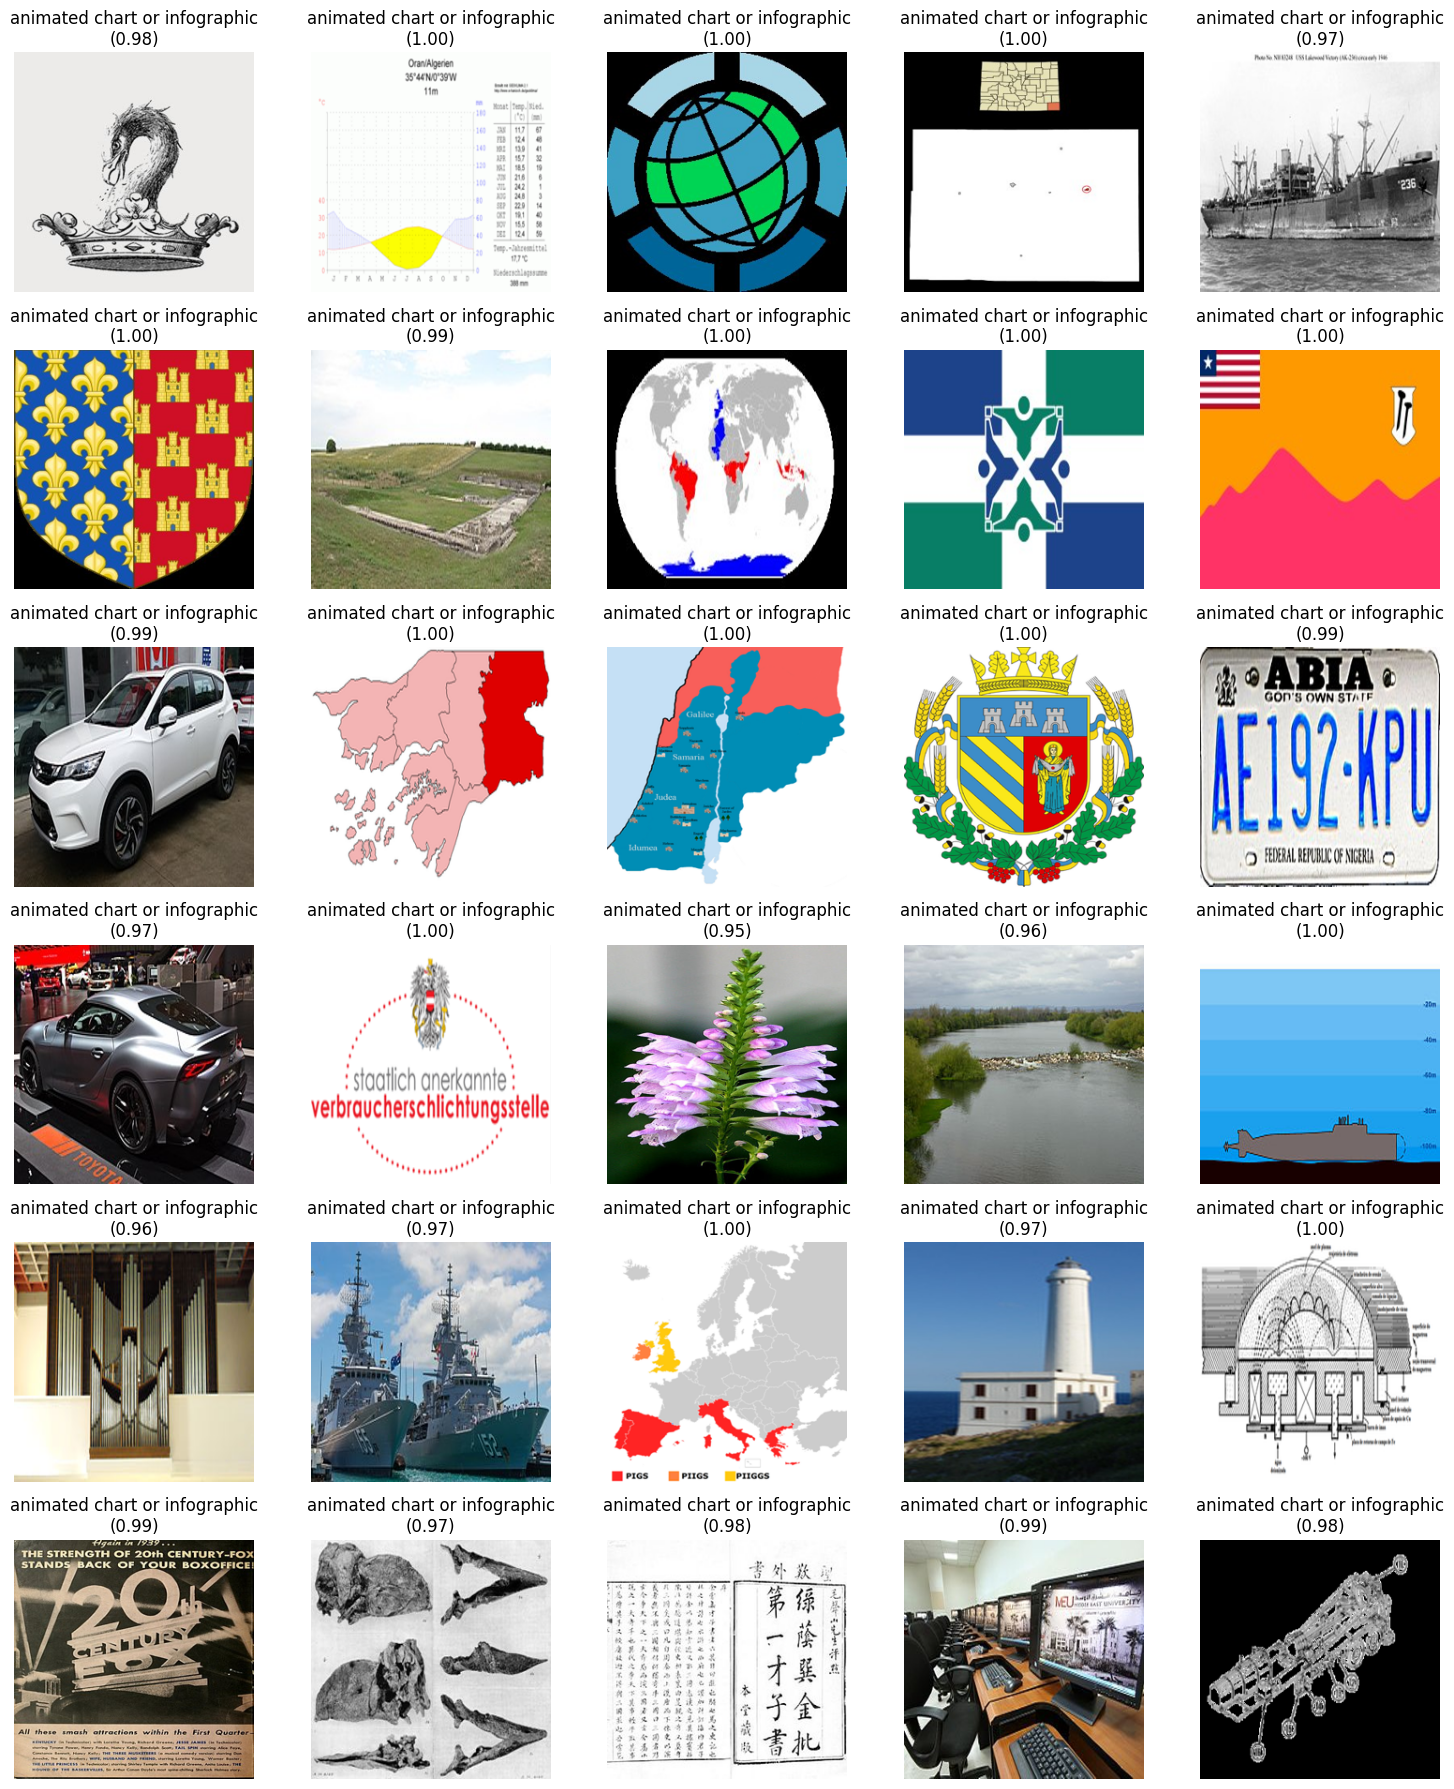
\includegraphics[width=0.4\textwidth]{images/zero-shot.png}
    \caption{Images removed by zero-shot classifier. Most of them introduces noise to the dataset, with acceptable FAR as a image to delete.}
\end{figure}

\section{Models}
\label{sec:models}

All following experiments were performed using \textbf{transformers} liblary from Hugging Face, which provides a wide range of pre-trained models and tools for fine-tuning them. All models were trained under $12$ hours each on $Nvidia 1060 6GB$ GPU, with batch size of $32$ and starting learning rate of $1e-4$ with cosine learning rate scheduler. Early stopping with $5$ epochs patience was used to prevent overfitting, with loading back to best model. Weight decay of $0.01$ was used to prevent overfitting as well. For hardware optimization, fp16 was used, which allows for faster training and lower memory usage. All models after each epoch were validated on the validation set, besides validation loss also metrics like accuracy, precision, recall and F1 score were calculated. Each model was trained on other datasets, which were described in section \ref{sec:datasets}, then on artificial dataset created based on WIT images.

Subsections containing results of training on our dataset show models that were first trained on other datasets, then on our (wit) dataset.

\subsection{\href{https://huggingface.co/blog/rwightman/mobilenetv4}{mobile net v4}}

MobileNetV4 is a lightweight convolutional neural network designed for mobile and edge device applications. This model focuses on reducing computational cost while maintaining high accuracy, achieved through a combination of:

\begin{figure}[H]
    \centering
    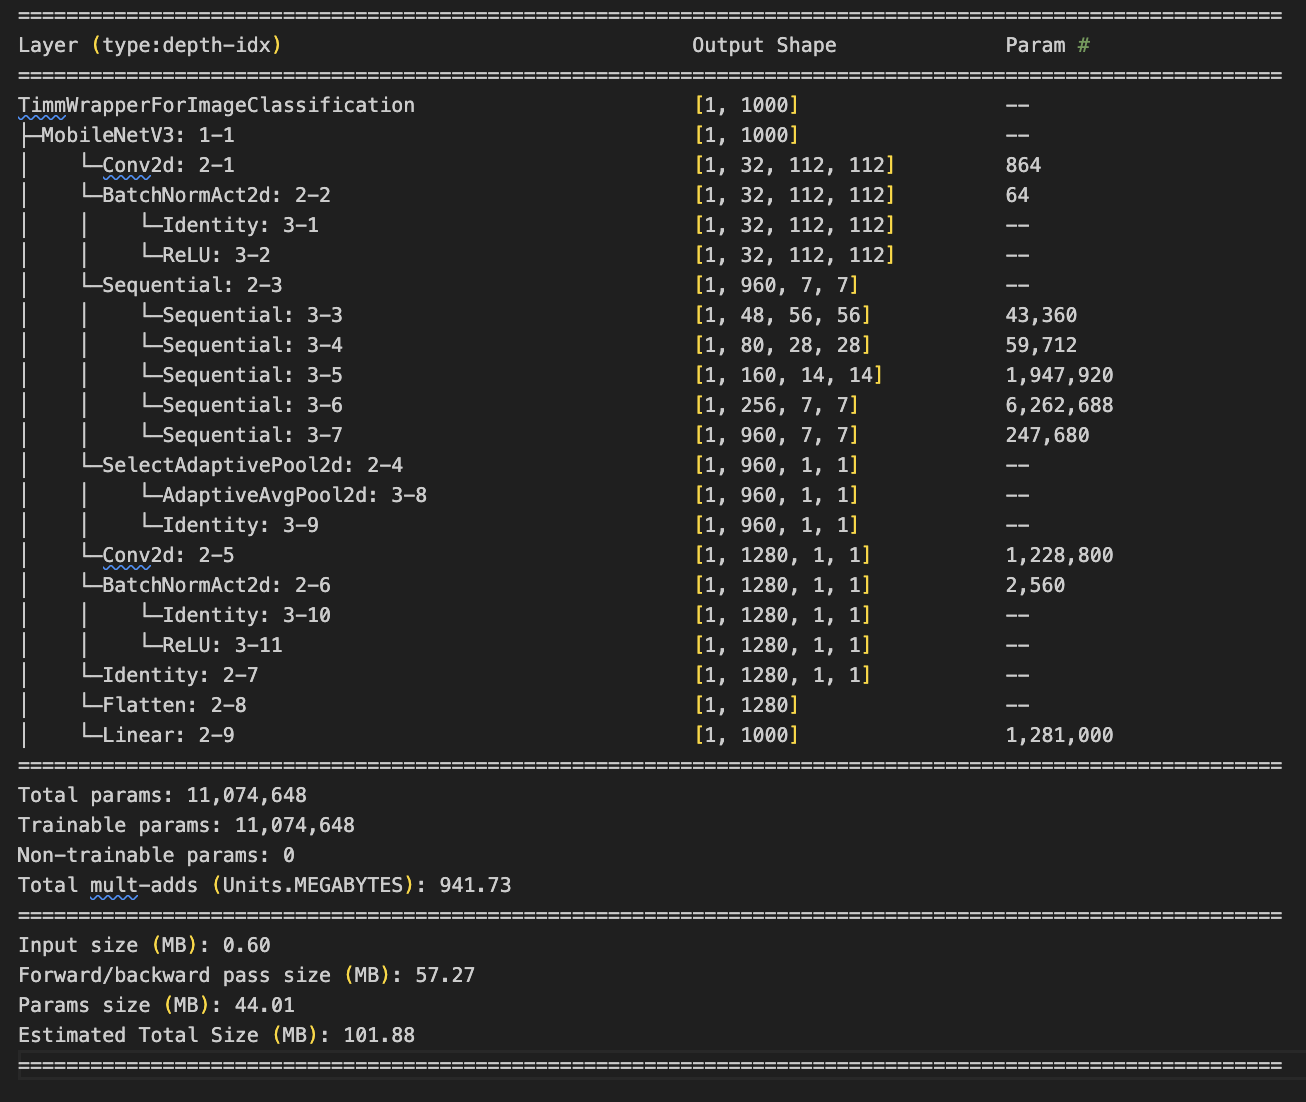
\includegraphics[width=0.5\textwidth]{images/mobile-net.png}
    \caption{Mobile Net specs for input size of $224\times224$.}
\end{figure}

\subsubsection{Other datasets}

\begin{table}[H]
    \centering
    \caption{Training progress of Mobile Net V4 model. Total $15$ epochs after early stopping with patience of $5$ epochs. Total training time $141$ minutes.}
    \label{tab:mobile_net_training_progress}
    \begin{tabular}{ccccccc}
        \toprule
        \textbf{Epoch} & \textbf{Training Loss} & \textbf{Validation Loss} & \textbf{Accuracy} & \textbf{Precision} & \textbf{Recall} & \textbf{F1} \\
        \midrule
        1  & 0.132300 & 0.180474 & 0.958206 & 0.959881 & 0.958206 & 0.958023 \\
        2  & 0.086600 & 0.110209 & 0.959948 & 0.962068 & 0.959948 & 0.960037 \\
        3  & 0.076400 & 0.065332 & 0.980192 & 0.980294 & 0.980192 & 0.980204 \\
        4  & 0.067100 & 0.050342 & 0.985633 & 0.985637 & 0.985633 & 0.985635 \\
        5  & 0.061300 & 0.074897 & 0.976926 & 0.977269 & 0.976926 & 0.976952 \\
        6  & 0.052900 & 0.041778 & 0.986069 & 0.986116 & 0.986069 & 0.986060 \\
        7  & 0.058400 & 0.064377 & 0.988681 & 0.988691 & 0.988681 & 0.988683 \\
        8  & 0.051700 & 0.042357 & 0.987810 & 0.987810 & 0.987810 & 0.987809 \\
        9  & 0.056900 & 6.401874 & 0.603396 & 0.726450 & 0.603396 & 0.506545 \\
        10 & 0.036900 & 0.033462 & 0.989769 & 0.989794 & 0.989769 & 0.989765 \\
        11 & 0.041700 & 0.054621 & 0.986939 & 0.987029 & 0.986939 & 0.986947 \\
        12 & 0.039700 & 0.145202 & 0.984545 & 0.984552 & 0.984545 & 0.984540 \\
        13 & 0.038600 & 0.569320 & 0.987593 & 0.987699 & 0.987593 & 0.987601 \\
        14 & 0.037100 & 0.210024 & 0.987375 & 0.987390 & 0.987375 & 0.987378 \\
        15 & 0.033400 & 0.039065 & 0.989987 & 0.990080 & 0.989987 & 0.989979 \\
        \bottomrule
    \end{tabular}
\end{table}

\begin{table}[H]
    \centering
    \caption{Evaluation metrics of Mobile Net V4 model on other datasets (rest) and WIT dataset (wit).}
    \label{tab:mobile_net_eval}
    \begin{tabular}{lcc}
        \toprule
        \textbf{Metric} & \textbf{Other Datasets (rest)} & \textbf{WIT Dataset (wit)} \\
        \midrule
        Validation Loss      & 0.02697   & 0.86145 \\
        Accuracy             & 0.99021   & 0.71160 \\
        Precision            & 0.99022   & 0.78528 \\
        Recall               & 0.99021   & 0.71160 \\
        F1 Score             & 0.99020   & 0.72056 \\
        Runtime (s)          & 28.79     & 58.83 \\
        Samples/sec          & 159.63    & 169.99 \\
        Steps/sec            & 5.00      & 5.32 \\
        Epoch                & 15        & 15 \\
        \bottomrule
    \end{tabular}
\end{table}

\subsubsection{Our (wit) dataset}

\begin{table}[H]
    \centering
    \caption{Training progress of Mobile Net V4 model on WIT dataset. Total $14$ epochs after early stopping with patience of $3$ epochs. Total training time $314$ minutes.}
    \label{tab:mobile_net_wit_training_progress}
    \begin{tabular}{ccccccc}
        \toprule
        \textbf{Epoch} & \textbf{Training Loss} & \textbf{Validation Loss} & \textbf{Accuracy} & \textbf{Precision} & \textbf{Recall} & \textbf{F1} \\
        \midrule
        1  & 0.109900 & 0.092464 & 0.963800 & 0.964340 & 0.963800 & 0.963942 \\
        2  & 0.095500 & 0.065102 & 0.976700 & 0.976756 & 0.976700 & 0.976721 \\
        3  & 0.086800 & 0.069809 & 0.975800 & 0.975874 & 0.975800 & 0.975693 \\
        4  & 0.078100 & 0.084138 & 0.969700 & 0.970194 & 0.969700 & 0.969440 \\
        5  & 0.079600 & 0.062597 & 0.976000 & 0.976041 & 0.976000 & 0.975905 \\
        6  & 0.072900 & 0.078142 & 0.972300 & 0.972758 & 0.972300 & 0.972077 \\
        7  & 0.076400 & 0.057125 & 0.979300 & 0.979284 & 0.979300 & 0.979290 \\
        8  & 0.073800 & 0.055456 & 0.982300 & 0.982282 & 0.982300 & 0.982274 \\
        9  & 0.073000 & 0.070988 & 0.980100 & 0.980077 & 0.980100 & 0.980083 \\
        10 & 0.057400 & 0.049798 & 0.983600 & 0.983585 & 0.983600 & 0.983577 \\
        11 & 0.060300 & 0.044705 & 0.984000 & 0.984021 & 0.984000 & 0.984008 \\
        12 & 0.061200 & 0.122837 & 0.973800 & 0.973793 & 0.973800 & 0.973711 \\
        13 & 0.058400 & 3.908190 & 0.952700 & 0.953347 & 0.952700 & 0.952890 \\
        14 & 0.071700 & 0.058245 & 0.980600 & 0.980718 & 0.980600 & 0.980514 \\
        \bottomrule
    \end{tabular}
\end{table}

\begin{table}[H]
    \centering
    \caption{Evaluation metrics of Mobile Net V4 model on other datasets (rest) and WIT dataset (wit).}
    \label{tab:mobile_net_wit_eval}
    \begin{tabular}{lcc}
        \toprule
        \textbf{Metric} & \textbf{Other Datasets (rest)} & \textbf{WIT Dataset (wit)} \\
        \midrule
        Validation Loss      & 0.49886   & 0.04635 \\
        Accuracy             & 0.89293   & 0.98340 \\
        Precision            & 0.89632   & 0.98344 \\
        Recall               & 0.89293   & 0.98340 \\
        F1 Score             & 0.89191   & 0.98342 \\
        Runtime (s)          & 29.09     & 61.24 \\
        Samples/sec          & 157.97    & 163.29 \\
        Steps/sec            & 4.95      & 5.11 \\
        Epoch                & 14        & 14 \\
        \bottomrule
    \end{tabular}
\end{table}

\subsection{\href{https://huggingface.co/blog/siglip2}{siglip 2}}

The siglip2 model is a multilingual vision-language encoder. It is larger to mobile net v4, but it is still lightweight and efficient. It was trained with expectation to exceedee performance of mobile net v4 on image classification tasks, as a better yet heavier alternative.

After studying of below training progress, it can be concluded that it is unable to overcome performance of 1st epoch. It is however important to point out that both datasets contain large number of images and there is a possibility that model learns majority of their variance within steps of first epoch, further training leads to destruction of apriori knowledge from imagenet thus leading to worse performance.

\begin{figure}[H]
    \centering
    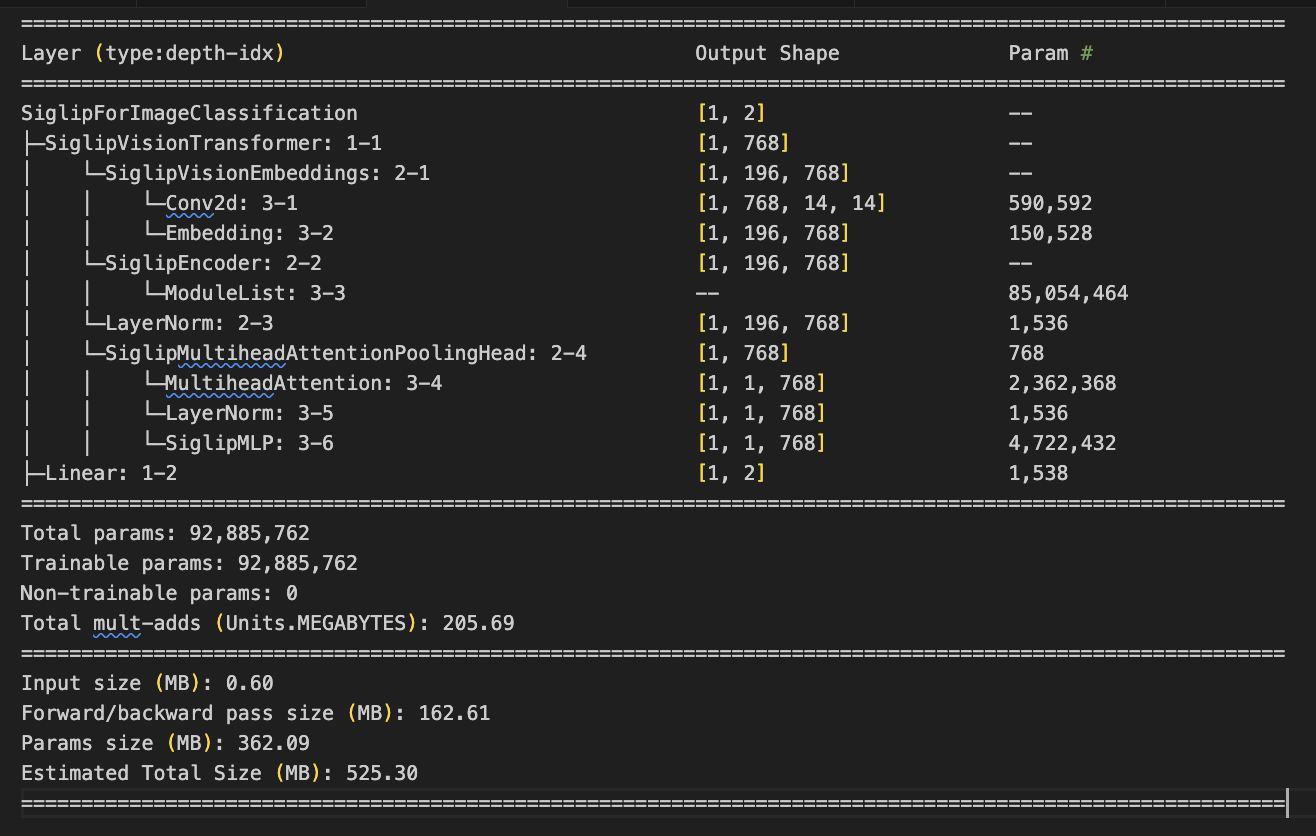
\includegraphics[width=0.5\textwidth]{images/siglip.png}
    \caption{Siglip specs for input size of $224\times224$.}
\end{figure}

\subsubsection{Other datasets}

\begin{table}[H]
    \centering
    \caption{Training progress of Siglip 2 model on other datasets. Total $6$ epochs after early stopping with patience of $5$ epochs. Total training time $820$ minutes.}
    \label{tab:siglip_training_progress}
    \begin{tabular}{ccccccc}
        \toprule
        \textbf{Epoch} & \textbf{Training Loss} & \textbf{Validation Loss} & \textbf{Accuracy} & \textbf{Precision} & \textbf{Recall} & \textbf{F1} \\
        \midrule
        1 & 0.359900 & 0.292432 & 0.885503 & 0.891092 & 0.885503 & 0.885800 \\
        2 & 0.336200 & 0.388499 & 0.823901 & 0.851418 & 0.823901 & 0.816936 \\
        3 & 0.359900 & 0.366436 & 0.833914 & 0.837699 & 0.833914 & 0.832022 \\
        4 & 0.381300 & 0.406820 & 0.815629 & 0.822322 & 0.815629 & 0.816095 \\
        5 & 0.382600 & 0.404702 & 0.819983 & 0.823476 & 0.819983 & 0.820429 \\
        6 & 0.388600 & 0.403304 & 0.810623 & 0.814234 & 0.810623 & 0.808270 \\
        \bottomrule
    \end{tabular}
\end{table}

\begin{table}[H]
    \centering
    \caption{Evaluation metrics of Siglip 2 model on other datasets and WIT dataset.}
    \label{tab:siglip_eval}
    \begin{tabular}{lcc}
        \toprule
        \textbf{Metric} & \textbf{Other Datasets} & \textbf{WIT Dataset} \\
        \midrule
        Validation Loss      & 0.2899   & 0.3124 \\
        Accuracy             & 0.8860   & 0.8787 \\
        Precision            & 0.8928   & 0.8795 \\
        Recall               & 0.8860   & 0.8787 \\
        F1 Score             & 0.8864   & 0.8749 \\
        Runtime (s)          & 459.83   & 171.79 \\
        Samples/sec          & 9.99     & 58.21 \\
        Steps/sec            & 0.313    & 1.822 \\
        Epoch                & 6        & 6 \\
        \bottomrule
    \end{tabular}
\end{table}

\subsubsection{Our (wit) dataset}

\begin{table}[H]
    \centering
    \caption{Training progress of Siglip 2 model on WIT dataset. Total $4$ epochs after early stopping with patience of $3$ epochs. Total training time $484$ minutes minutes.}
    \label{tab:siglip_wit_training_progress}
    \begin{tabular}{ccccccc}
        \toprule
        \textbf{Epoch} & \textbf{Training Loss} & \textbf{Validation Loss} & \textbf{Accuracy} & \textbf{Precision} & \textbf{Recall} & \textbf{F1} \\
        \midrule
        1 & 0.204500 & 0.195957 & 0.918800 & 0.921943 & 0.918800 & 0.919573 \\
        2 & 0.245100 & 0.232362 & 0.904500 & 0.906685 & 0.904500 & 0.905179 \\
        3 & 0.281600 & 0.321944 & 0.870700 & 0.875127 & 0.870700 & 0.865230 \\
        4 & 0.255600 & 0.275362 & 0.885000 & 0.889506 & 0.885000 & 0.886241 \\
        \bottomrule
    \end{tabular}
\end{table}

\begin{table}[H]
    \centering
    \caption{Evaluation metrics of Siglip 2 model on other datasets (rest) and WIT dataset.}
    \label{tab:siglip_eval_4epochs}
    \begin{tabular}{lcc}
        \toprule
        \textbf{Metric} & \textbf{Other Datasets (rest)} & \textbf{WIT Dataset (wit)} \\
        \midrule
        Validation Loss      & 0.4837   & 0.1885 \\
        Accuracy             & 0.8359   & 0.9243 \\
        Precision            & 0.8400   & 0.9272 \\
        Recall               & 0.8359   & 0.9243 \\
        F1 Score             & 0.8337   & 0.9250 \\
        Runtime (s)          & 80.39    & 171.12 \\
        Samples/sec          & 57.16    & 58.44 \\
        Steps/sec            & 1.79     & 1.83 \\
        Epoch                & 4        & 4 \\
        \bottomrule
    \end{tabular}
\end{table}

\subsection{Conclusion}

Based on the results presented above, the \textbf{Mobile Net V4} model trained on the WIT dataset achieved the highest accuracy, reaching $98.34\%$ on the WIT dataset. This outperformed the \textbf{Siglip 2} model, which achieved $92.43\%$ accuracy on the same data. However, this improvement in F1 score on the WIT dataset was accompanied by a noticeable drop in performance on the other datasets. This suggests that the model may be overfitting to the WIT dataset or that the dataset itself may still contain some noise. Further investigation is required to better understand these results.

\end{document}
